\documentclass[smaller,professionalfonts,15pt]{beamer}
\usepackage{fontspec,unicode-math}
\usepackage{lipsum, lmodern}
\usepackage{polyglossia}
\usepackage{bncc}
\usepackage[lunna]{logoedlab}
\setdefaultlanguage{brazilian}
\usetheme[widescreen]{PraterStreet} 



\begin{document}


% Abertura -----------------------------------------------------------------
										\begin{frame}\begin{raggedleft}
										\Huge 
Crônicas e contos						\\
										\huge 
Lima Barreto							\\
										\bigskip
										\normalsize
Tema: Ficção, mistério e fantasia		\\	
Gênero: Conto, crônica e novela			\\\vfill\hfill
\publishername
										\end{raggedleft}

%\vspace{2cm}\includegraphics[width=4cm]{\logoeditora}
\end{frame}


% Logo ---------------------------------------------------------------------
\begin{frame}{\textsc{videotutorial para o professor sobre atividades}}
\vspace{-2cm}\begin{figure}
	\IfFileExists{PNLD0001-01.png}{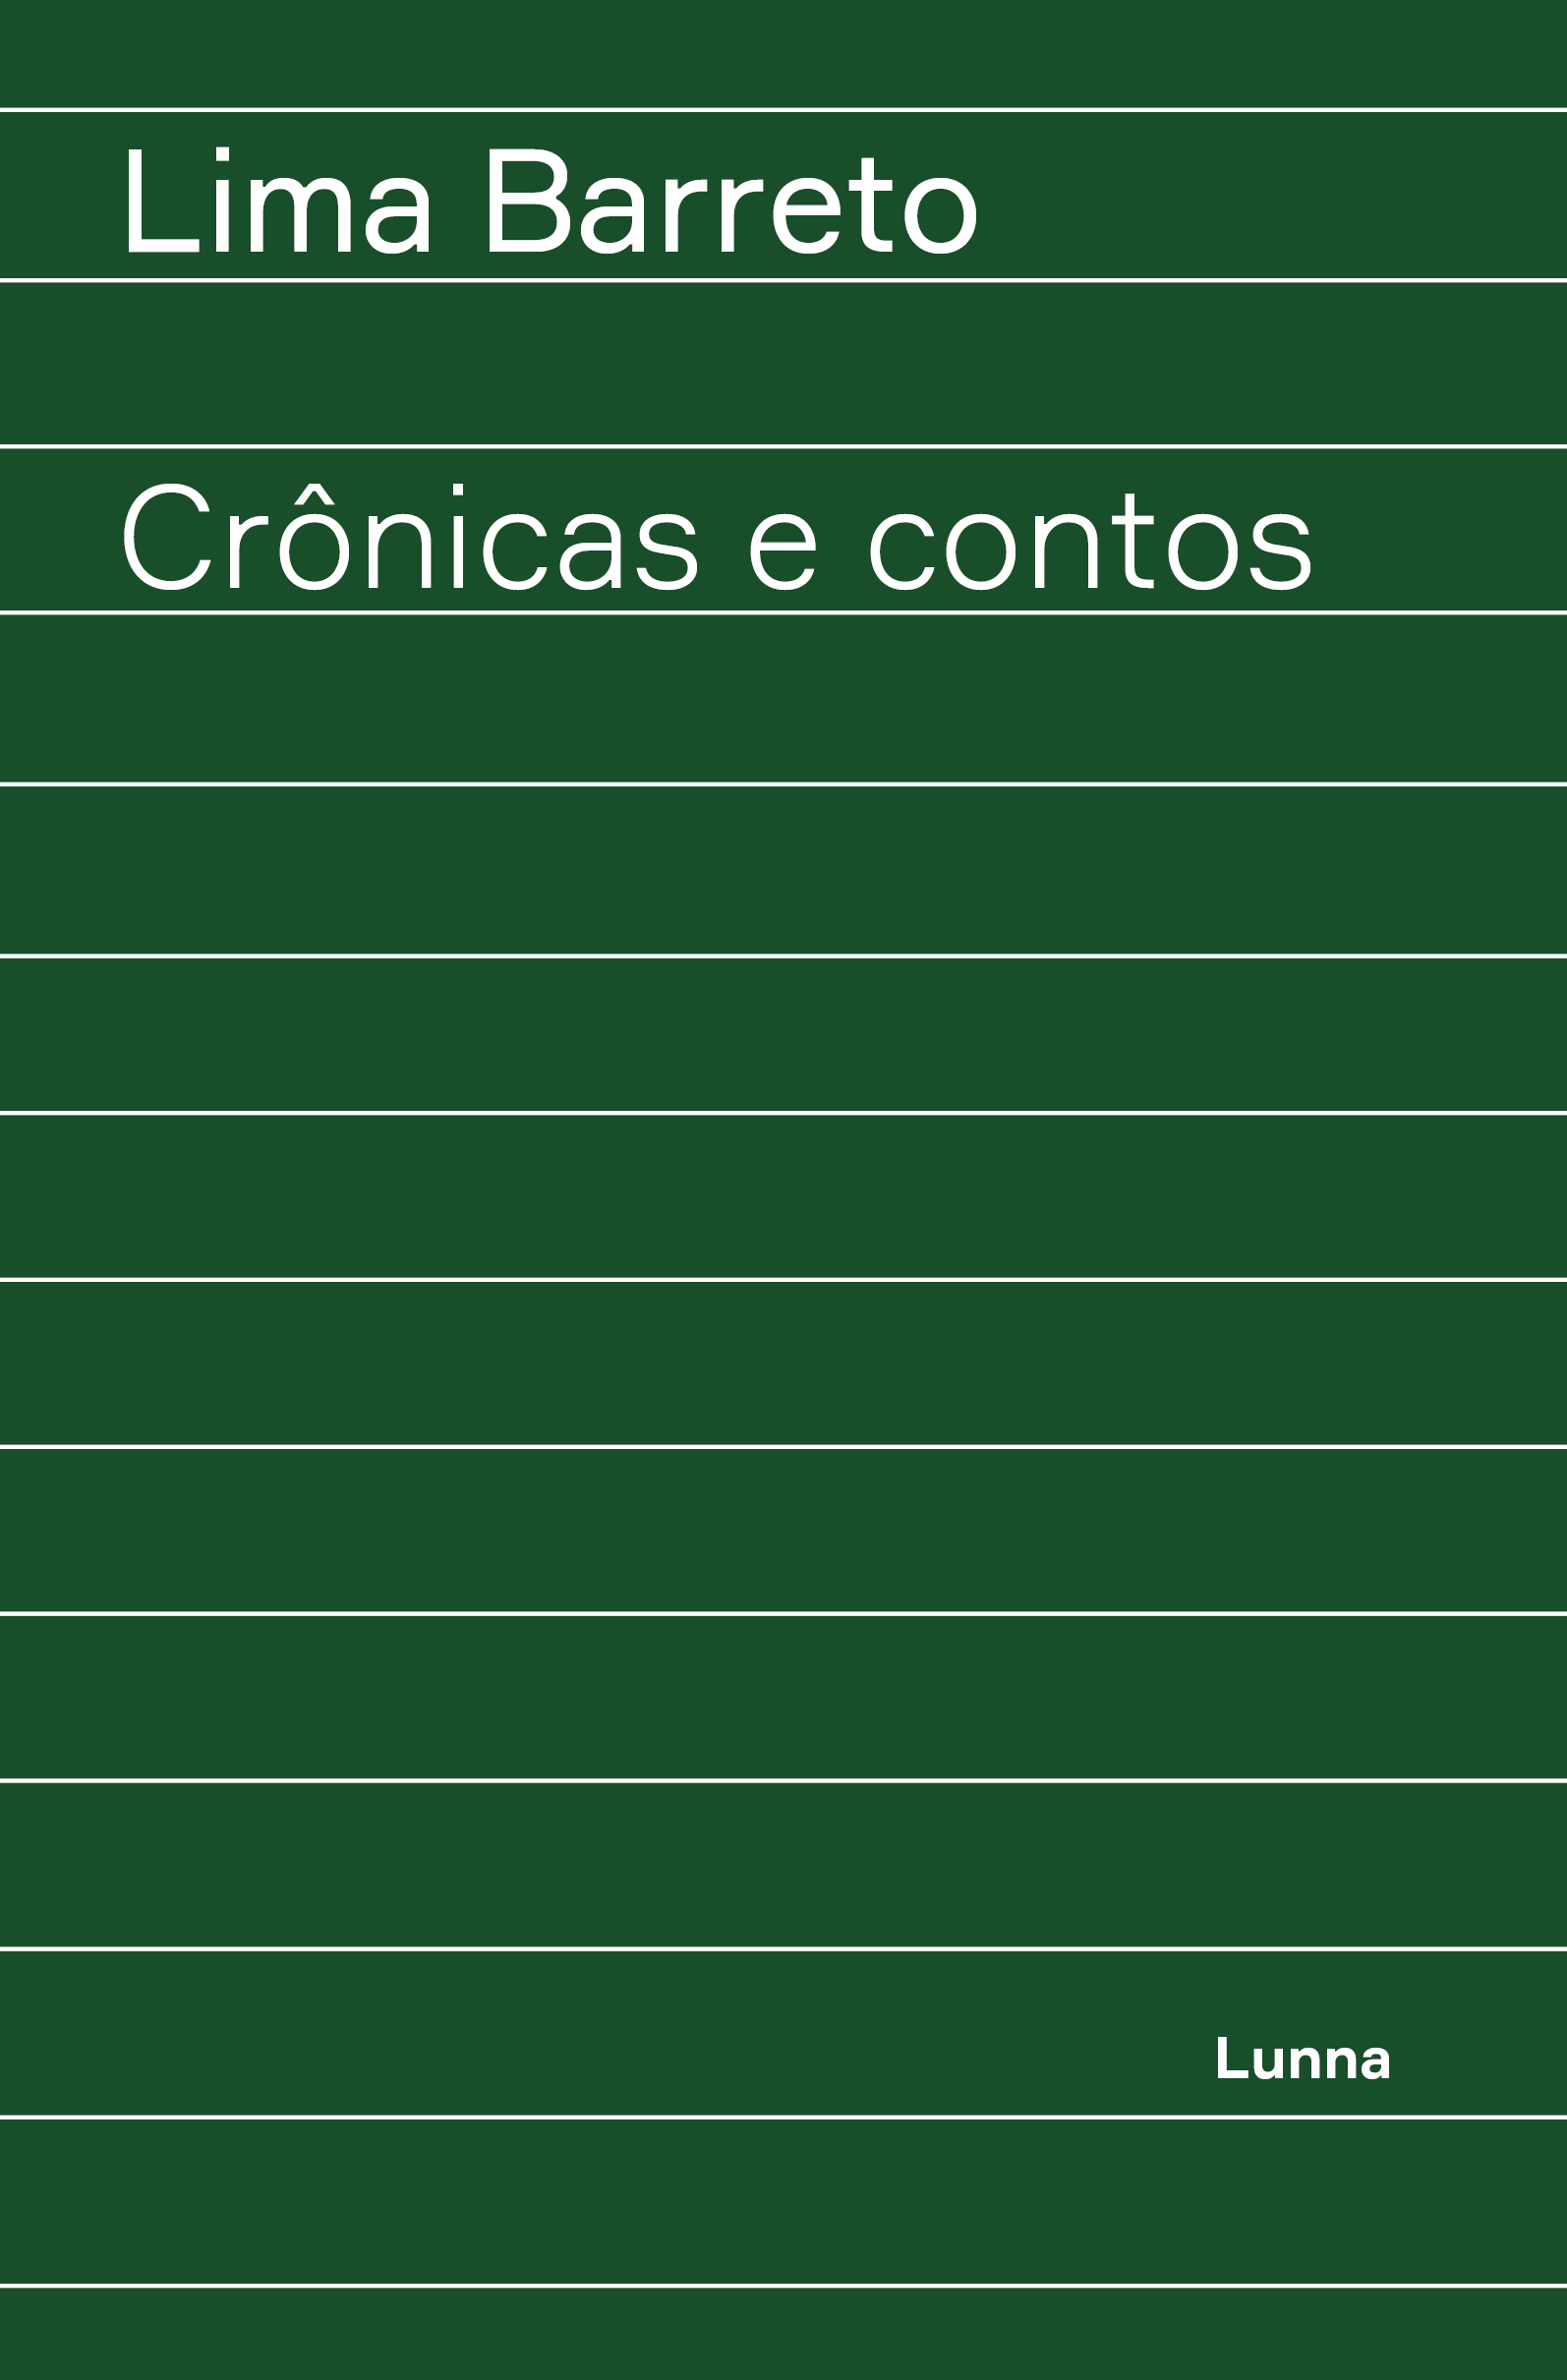
\includegraphics[width=5cm]{PNLD0001-01.png}}{Aplicar Capa!!}
\end{figure}
\end{frame}

% Slides -------------------------------------------------------------------

\begin{frame}
\hfill\Huge
\textsc{atividade 1}
\end{frame}


\begin{frame}
\hfill\Huge
\textsc{atividade 2}
\end{frame}

% BNCC ---------------------------------------------------------------------
\begin{frame}[plain]{Habilidades da BNCC para a Atividade 1}
\vspace{-2cm}
\BNCC{EM13LGG301}
\BNCC{EM13LGG401}
\BNCC{EM13LGG402}
\BNCC{EM13LGG703}
\BNCC{EM13LGG704}
\BNCC{EM13LP16}
\BNCC{EM13LP27}
\BNCC{EM13LP29}
\end{frame}

\begin{frame}[plain]{Habilidades da BNCC para a Atividade 1}
\vspace{-2cm}
\BNCC{EM13LP36}
\BNCC{EM13LP44}
\BNCC{EM13LP45}
\BNCC{EM13LP46}
\BNCC{EM13LP47}
\BNCC{EM13LP48}
\BNCC{EM13LP50}
\BNCC{EM13LP53}

\end{frame}

\begin{frame}[plain]{Habilidades da BNCC para a Atividade 2}
\vspace{-2cm}
\BNCC{EM13LGG703}
\BNCC{EM13LGG704}
\BNCC{EM13LP16}
\BNCC{EM13LP36}
\BNCC{EM13LP44 }
\BNCC{EM13CHS501}
\BNCC{EM13CHS502}
\BNCC{EM13CHS503}
\BNCC{EM13CHS504}
\BNCC{EM13CHS601}

\end{frame}

% Fechamento ---------------------------------------------------------------
\setbeamertemplate{background}{%
		\includegraphics[width=\paperwidth, 
		height=\paperheight, 
		keepaspectratio]{BGW.pdf}}

\begin{frame}
\centering\hfill\includegraphics[width=7cm]{\logoeditora}
\end{frame}

\end{document}
